\let\negmedspace\undefined
\let\negthickspace\undefined
\documentclass[journal]{IEEEtran}
\usepackage[a5paper, margin=10mm, onecolumn]{geometry}
%\usepackage{lmodern} % Ensure lmodern is loaded for pdflatex
\usepackage{tfrupee} % Include tfrupee package

\setlength{\headheight}{1cm} % Set the height of the header box
\setlength{\headsep}{0mm}     % Set the distance between the header box and the top of the text
\usepackage{multicol}
\usepackage{gvv-book}
\usepackage{gvv}
\usepackage{cite}
\usepackage{amsmath,amssymb,amsfonts,amsthm}
\usepackage{algorithmic}
\usepackage{graphicx}
\usepackage{textcomp}
\usepackage{xcolor}
\usepackage{txfonts}
\usepackage{listings}
\usepackage{enumitem}
\usepackage{mathtools}
\usepackage{gensymb}
\usepackage{comment}
\usepackage[breaklinks=true]{hyperref}
\usepackage{tkz-euclide} 
\usepackage{pgfplots}
\pgfplotsset{compat=1.18}
\usepackage{listings}
% \usepackage{gvv}                                        
\def\inputGnumericTable{}                                 
\usepackage[latin1]{inputenc}                                
\usepackage{color}                                            
\usepackage{array}                                            
\usepackage{longtable}                                       
\usepackage{calc}                                             
\usepackage{multirow}                                         
\usepackage{hhline}                                           
\usepackage{ifthen}                                           
\usepackage{lscape}
\usepackage{tikz}
% Marks the beginning of the document
\begin{document}
\bibliographystyle{IEEEtran}
\vspace{3cm}

\title{\\NCERT-11.16.3.17.2}
\author{EE24BTECH11056 - S.Kavya Anvitha}
\maketitle
%\newpage
\bigskip

\renewcommand{\thefigure}{\theenumi}
\renewcommand{\thetable}{\theenumi}
\section*{Problem:}
Given that:
\begin{itemize}
    \item $P(A) = 0.42$
    \item $P(B) = 0.48$
    \item $P(A \cap B) = 0.16$
\end{itemize}
Find $P(B')$.

\textbf{Theoretical Solution:}\\
For two Boolean variables \( A \) and \( B \), we use the axiom:
\begin{align}
B+B'=1\\
P(1)=1\\
P(B)+P(B')=1\\
  P(B') = 1 - P(B)  
\end{align}

Given:
\[
P(A) = 0.42, \quad P(B) = 0.48, \quad P(A \cap B) = 0.16
\]
Using the formula:
\begin{align}
 P(B') = 1 - 0.48 = 0.52   
\end{align}


Thus, \( P(B') = 0.52 \).

\vspace{1cm}

\textbf{Computational Solution:}\\
Define indicator random variable:

\begin{itemize}
    \item \( X \) for event \( B' \)
\end{itemize}



Let \( X \) be an indicator random variable for \( B' \):

\begin{align}
X =
\begin{cases}
1 ,& B'\\
0 ,& B
\end{cases}
\end{align}
The probability mass function (PMF) for \( X \) (representing the event \( B' \)):

\begin{align}
p_{X}(n) =
\begin{cases}
1 - p ,& n = 1\\
p ,& n = 0
\end{cases}
\end{align}
where \( p = P(B) = 0.48 \).\\
the PMF is:

\begin{align}
p_{X}(n) =
\begin{cases}
0.52 ,& n = 1 \\
0.48 ,& n = 0
\end{cases}
\end{align}

Thus, \( P(B') = 0.52 \).

\begin{figure}[h!]
   \centering
   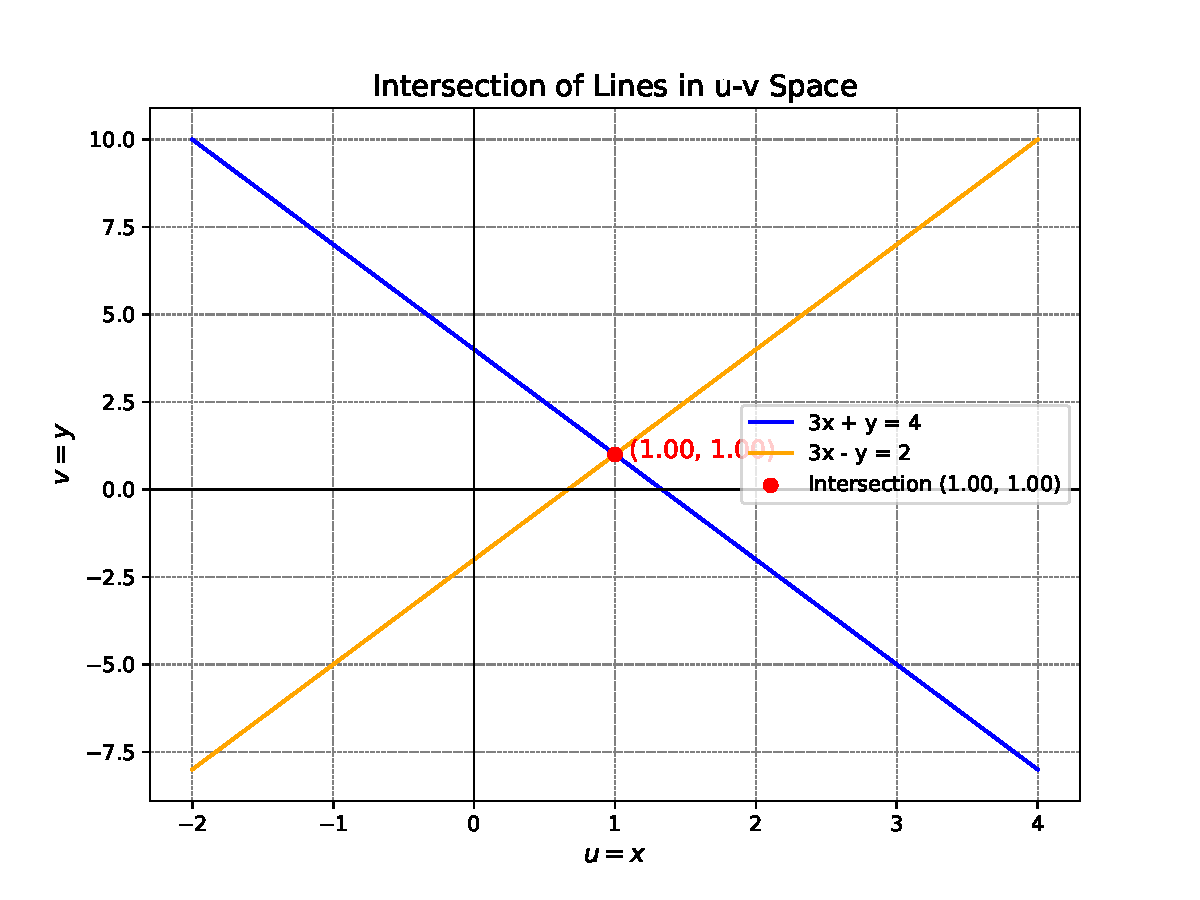
\includegraphics[width=\columnwidth]{figs/fig.pdf}
\end{figure}



\end{document}
